\documentclass[12pt,letterpaper,noanswers]{exam}
\usepackage[usenames,dvipsnames,svgnames,table]{xcolor}
\usepackage[margin=0.9in]{geometry}
\renewcommand{\familydefault}{\sfdefault}
\usepackage{multicol}
\usepackage{wrapfig}
\pagestyle{head}
\definecolor{c03}{HTML}{FFDDDD}
\header{AM 22b Class 07}{}{Feb 10: partial derivative, derivative, gradient}
\runningheadrule
\headrule
\usepackage{graphicx} % more modern
\usepackage{amsmath} 
\usepackage{amssymb} 
\usepackage{hyperref}
\usepackage{tcolorbox}

\usepackage[numbered,autolinebreaks,useliterate]{mcode}

\newcommand{\mb}[1]{\underline{#1}}

\begin{document}
 \pdfpageheight 11in 
  \pdfpagewidth 8.5in




% I need to review the torus trajectories...

\begin{itemize}
% \item There is a pre-class assignment (20 minutes of videos + a few WeBWorK exercises) due at 10am this Monday.  It is available on Canvas.
\itemsep0em
    \item There is a skill check on Friday (skills C06 and C07). 
    \item PSet 02 is due on Thursday Feb 10th at 6pm.
    \item There is a quiz next Friday (available through the weekend).  It is self-scheduled and will be administered via Gradescope.
\end{itemize}

\hrule
\vspace{0.2cm}

% partial derivatives, gradient
% local linearity, differential, directional deriv
% 2nd order partials + equations with partials

\noindent\textbf{Big picture}

This week we are studying differentiation.  The focus is on rates of change given that we now have functions with multiple inputs and with multiple outputs.  One application of these ideas is optimization (which was a topic in 22a, and is not in 22b).  This background knowledge will also be used in our integration and vector calculus units.

\vspace{0.2cm}
\hrule
\vspace{0.2cm}

\noindent\textbf{Skill Check C07 practice}

Construct $D \mb{f}$ for the function $\displaystyle\mb{f} =  \left(\begin{array}{c}xze^y \\ x^2 + xyz \end{array}\right)$.

\vspace{0.2cm}
\hrule
\vspace{0.2cm}

\noindent\textbf{Skill Check C07 solution}

$D \mb{f}$ is the Jacobian matrix.  The function has three inputs and two outputs, so the Jacobian will be a 2x3 matrix (two rows and three columns).  Finding the six partials, we have $D\mb{f} = \left(\begin{array}{c c c}ze^y & x z e^y & xe^y \\ 2x + yz & xz & xy \end{array}\right)$

\vspace{0.2cm}
\hrule
\vspace{0.2cm}

\noindent\textbf{Teams}

You will work with this team on in-class problems today.  Introduce yourself to your new team.
\begin{multicols}{2}
1.  student names

\end{multicols}

%\vspace{0.2cm}
\hrule
\vspace{0.2cm}

\noindent\textbf{What are derivatives for?}

\begin{itemize}
\itemsep0em
    \item description: what is the sensitivity of this quantity to change in another quantity? how fast is this changing?; 
    Examples:
    \begin{itemize}
        \item cardiac health measurement (``distensibility coefficient''): rate of change of arterial diameter with change in pulse pressure.  i.e. how much the artery distends during the heartbeat \cite{reneman1986age}
        \item rate of change of image intensity with position for edge detection in images \cite{torre1986edge}
        \item rate of change of flavor with respect to an ingredient (i.e. will the soup taste better or worse if I add a little salt). 
    \end{itemize}
        
    \item prediction: what might happen in the future? (differential equation modeling).
    
    Example:
    \begin{itemize}
        \item Predicting future position of an object to improve motion tracking.  \cite{hu2004survey}
    \end{itemize}
    
    \item control: given a mathematical description of the evolution of a system, and a set of possible interventions, how can the state of the system be guided to a desired state?
    
     Example:
    \begin{itemize}
        \item Controlling glucose levels with continuous glucose monitoring by using the rate of change to predict levels in the future.  \cite{klonoff2017simplified}
    \end{itemize}
\end{itemize}

\vspace{0.2cm}
\hrule
\vspace{0.2cm}

\noindent\textbf{Single variable derivative facts}

\begin{tcolorbox}

The \textbf{average rate of change} of a function $f(x)$ over the interval from $a$ to $a+h$ is given by $ \frac{f(a+h) - f(a)}{h}.$  The dimensions of this average rate are given by $\frac{[f(x)]}{[x]}$.

The \textbf{instantaneous rate of change} of a function $f(x)$ at the point $a$ is given by $ \lim\limits_{h\rightarrow 0} \frac{f(a+h) - f(a)}{h}.$  This is the \textbf{derivative} of $f$ at $a$, denoted $\frac{df}{dx}(a)$, $\left.\frac{df}{dx}\right\vert_a$, or $f'(a)$.  The dimensions of this instantaneous rate are given by $\frac{[f(x)]}{[x]}$.

When $h$ is sufficiently close to $0$, the average rate of change of $f(x)$ at a point $a$ serves as an \textbf{approximation} to the derivative of $f$ at $a$.
\end{tcolorbox}

\noindent\textbf{Example.}
\begin{itemize}
    \item $\frac{f(1+0.1)-f(1)}{0.1}$ is an approximation of $f'(1).$  $\frac{f(1+0.01)-f(1)}{0.01}$ is a better approximation of $f'(1)$.
\item Find three different approximations to the derivative of $f(x) = x^2$ at $x = 2$ using the function values in the following table

\begin{tabular}{|c| c|}
\hline
$x$ & $x^2$\\
\hline
\hline
2 & 4 \\
2.01 & 4.0401 \\
2.1 & 4.41 \\
2.5 & 6.25 \\
\hline
\end{tabular}

\end{itemize}

\vspace{0.2cm}
\hrule
\vspace{0.2cm}


%\eject

\noindent\textbf{Partial derivatives} \S 14.1
\begin{tcolorbox}
To generalize the instantaneous rate of change to a multivariable context, we take \textbf{partial derivatives} along cross sections of the function.  Given a function $f(x,y)$, $f:\mathbb{R}^2 \rightarrow \mathbb{R}$,
\begin{itemize}
\item The notation $\frac{\partial f}{\partial x}(a,b)$ means ``Set $y=b$ and find the partial derivative with respect to $x$ at $x=a$.''  $\left.\frac{\partial f}{\partial x}\right\vert_{(a,b)} =  \lim\limits_{h\rightarrow 0} \frac{f(a+h,b) - f(a,b)}{h}.$  This partial derivative will also be denoted $f_x(a,b)$.
\item We can also compute the partial with respect to $y$: $\left.\frac{\partial f}{\partial y}\right\vert_{(a,b)} =  \lim\limits_{h\rightarrow 0} \frac{f(a,b+h) - f(a,b)}{h}.$ 
\end{itemize}

The symbol $\partial$ (see \url{https://en.wikipedia.org/wiki/%E2%88%82}) is used to distinguish partial derivatives from ordinary ones (or sometimes from total derivatives).  (Random fact: Legendre, inventor of the symbol, and Jacobi, key user of the symbol, each have a moon crater named for them.)

The \textbf{dimension} associated with a partial derivative is the dimension of the numerator divided by the dimension of the denominator.  Similarly, the \textbf{units} associated with the partial are the units of the numerator divided by the units of the denominator. If $w$ is a mass measured in kilograms and $x$ is a length measured in meters then the dimension of $\frac{\partial w}{\partial x}$ will be mass per length and the units will be kilograms per meter.


\end{tcolorbox}

\noindent\textbf{Example.}
\begin{enumerate}
    \item For the figure on the left below, assume you're looking at a graph.
    
    What is the input space of the function and what is its output space?
    
    Assume $A$ and $B$ are points in the $xy$-plane.
    
    What is the sign of $\left.\frac{\partial f}{\partial x}\right\vert_A$?

%% \includegraphics{C05fcn.pdf}
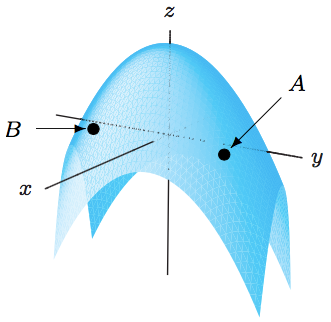
\includegraphics[width=1.5in]{img/C05ex2.png}
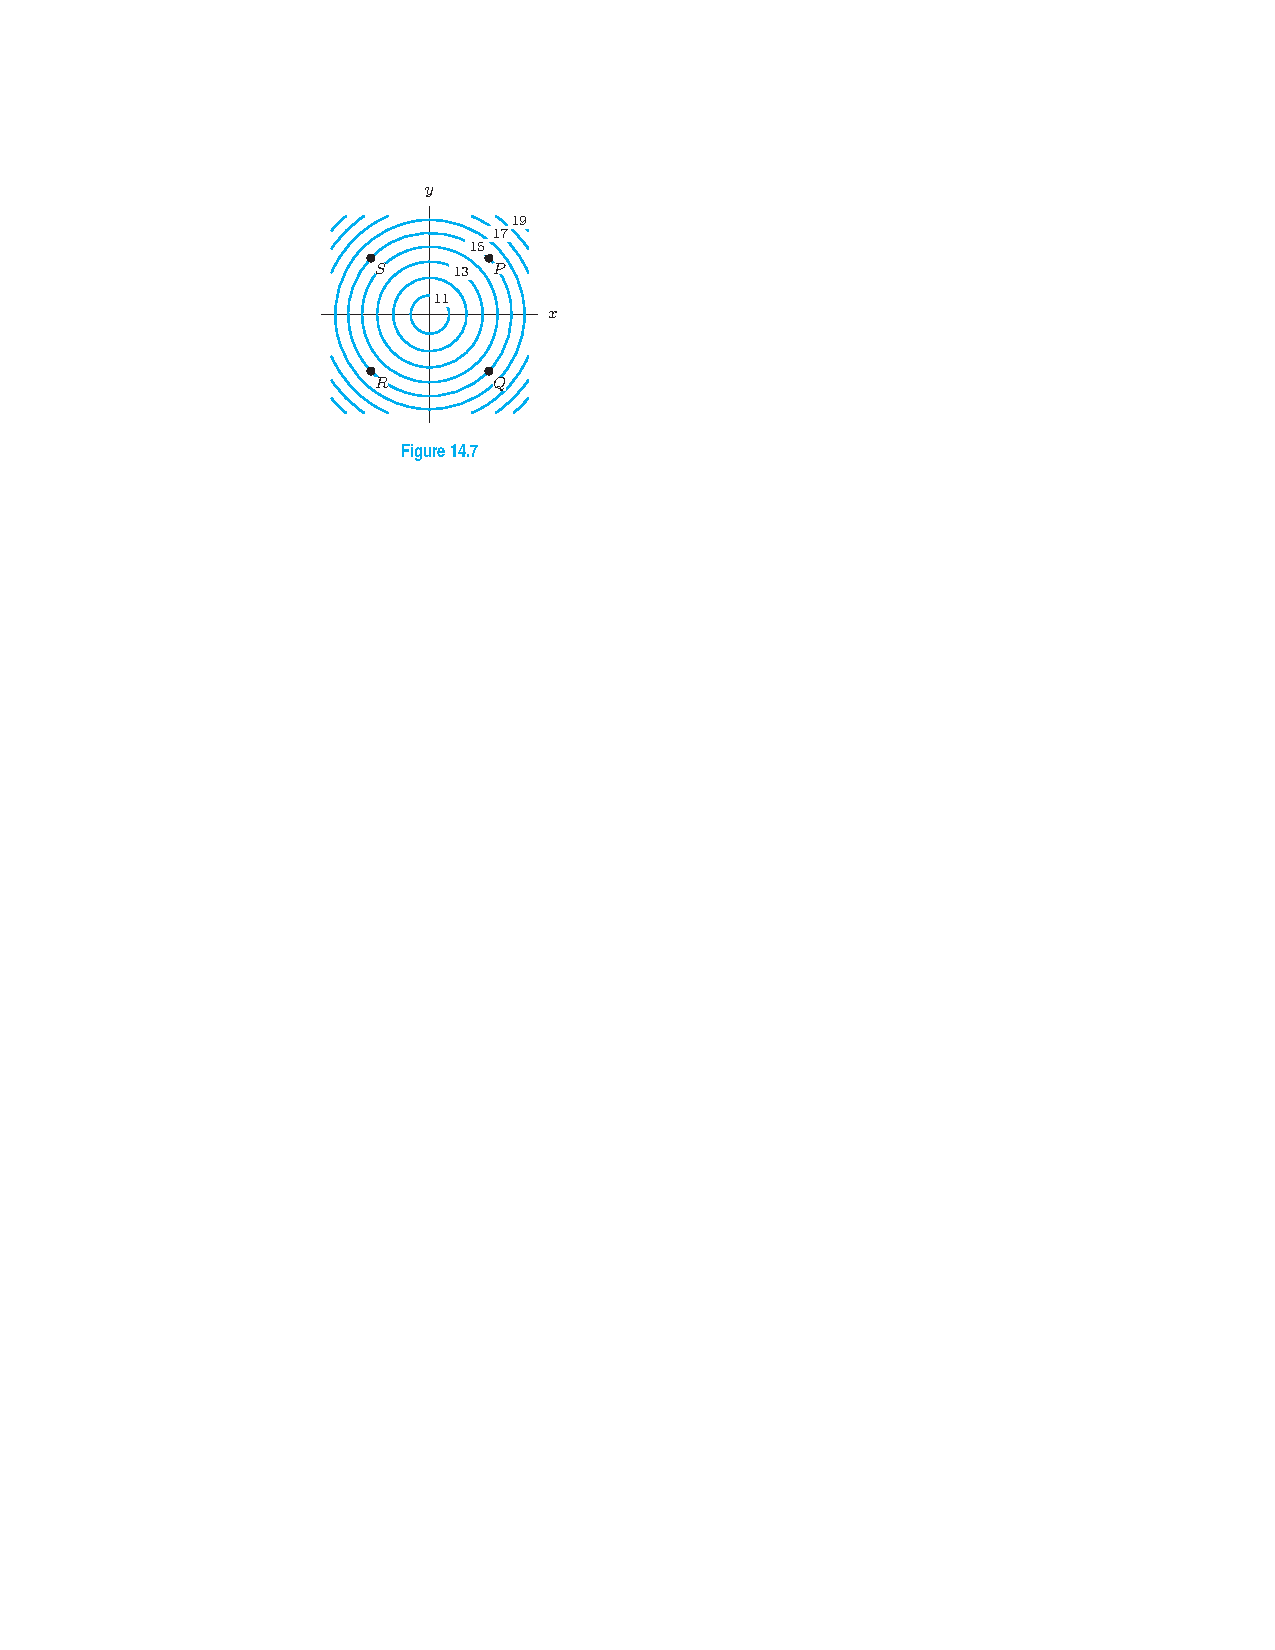
\includegraphics{img/C05ctr.pdf}



\item
For the figure on the right above, what is the input space of the function?  What is its output space?

What is the sign of $\left.\frac{\partial f}{\partial y}\right\vert_Q$?

What is the sign of $\left.\frac{\partial f}{\partial x}\right\vert_P$ ?

What is the sign of $\left.\frac{\partial f}{\partial y}\right\vert_P$?

%\item  From the info in the contour plot, Approximate the instantaneous rate of change $\left.\frac{\partial f}{\partial x}\right\vert_P$ using an average rate of change.

\item If possible, identify a point on the contour plot where $f_x < 0$ and $f_y<0$.  Explain your reasoning.
\end{enumerate}

\vspace{0.2cm}
\hrule
\vspace{0.2cm}

% \noindent\textbf{Example}

% \url{https://www.cambridgema.gov/-/media/Files/waterdepartment/labfiles/2019annualdrinkingwaterqualityreport.pdf}

% We can describe Cambridge's water quality as a vector-valued function, $\mb{f}$, where the vector consists of about 27 measured compounds.  

% Water quality depends on many factors.  The Cambridge water report identifies a number of sources of measured compounds: road salt, local mineral deposits, corrosion of plumbing, fertilizer runoff, compounds that are added for treatment, man-made chemicals.




% \vspace{0.2cm}
% \hrule
% \vspace{0.2cm}

%\eject

\noindent\textbf{Computing partial derivatives} \S 14.2

\begin{tcolorbox}
To \textbf{compute} a partial derivative with respect to $x$, treat other variables as constants. Compute an ordinary derivative with $x$ as the variable.

We can create a function $g_x(x,y)$ or $g_y(x,y)$.  These functions allow us to evaluate the partial derivative of $g$ with respect to $x$ (or to $y$) at any point $(x,y)$.

For a function $\mb{f}: \mathbb{R}^n\rightarrow\mathbb{R}^m$ where $\mb{x}\mapsto\mb{f}(\mb{x}),$ the \textbf{derivative} $Df$ or \textbf{Jacobian} matrix $\frac{\partial\mb{f}}{\partial \mb{x}}$ is given by the $m$ by $n$ matrix $\left(\begin{array}{c c c c}\frac{\partial f_1}{\partial x_1} & \frac{\partial f_1}{\partial x_2} & ... & \frac{\partial f_1}{\partial x_n} \\
\frac{\partial f_2}{\partial x_1} & \frac{\partial f_2}{\partial x_2} & ... & \frac{\partial f_2}{\partial x_n} \\
\vdots & \vdots & \ddots & \vdots \\
\frac{\partial f_m}{\partial x_1} & \frac{\partial f_m}{\partial x_2} & ... & \frac{\partial f_m}{\partial x_n} \\
\end{array}\right)$.  This is a \textbf{linear transformation} that can act on a vector of rates of change.  It transforms a vectors of rates of change for the input space of the function $\mb{f}$ to a vector of rates of change for the output space of $\mb{f}$.
\end{tcolorbox}
\begin{tcolorbox}
Consider a function $f:\mathbb{R}^n \rightarrow \mathbb{R}$.  The \textbf{gradient vector} for $f$ is the vector $\nabla f = \left(\begin{array}{c} \frac{\partial f}{\partial x_1} \\ \frac{\partial f}{\partial x_2} \\ \vdots \\ \frac{\partial f}{\partial x_n}\end{array}\right)$.  This is a vector.  It looks similar to $Df = \left(\begin{array}{c c c c}\frac{\partial f}{\partial x_1} & \frac{\partial f}{\partial x_2} & ... & \frac{\partial f}{\partial x_n}\end{array}\right)$, but $Df$ is a linear transformation, while $\nabla f$ is a vector.

The symbol $\nabla$ is called \textbf{del}, so $\nabla f$ can be read as ``del f'' or as ``grad f''.  \emph{Note that symbol by itself is \textbf{not} called ``grad'', so if it is used in other contexts you would say ``del''.}  The symbol is also sometimes called \textbf{nabla}.


\end{tcolorbox}

\noindent\textbf{Examples.}

\begin{enumerate}
\item Construct $Df$ for the function $\left(\begin{array}{c} x(r,\theta) \\ y(r,\theta) \end{array}\right) = \left(\begin{array}{c} r\cos\theta \\ r\sin\theta \end{array}\right)$.  This function has two inputs, $(r,\theta)$, and two outputs, $(x,y)$.
\vspace{0.7in}



\begin{lstlisting}
% Check in Matlab:
syms r t
jacrt = jacobian([r*cos(t),r*sin(t)],[r,t])
\end{lstlisting}

\item Find $\left.Df\right\vert_{(1,\pi/2)}$ for the function above.
\vspace{0.5in}


\begin{lstlisting}
% Check in Matlab:
subs(jacrt,[r,t],[1,pi/2])
\end{lstlisting}

\item Construct $Df$ for the function $f(x,y) = x^2y$.
\vspace{0.3in}

\begin{lstlisting}
val = jacobian(x^2*y,[x,y]);
size(val) % this is 1 by 2.
\end{lstlisting}

\item Construct $\text{grad} f$ for $f(x,y) = x^2y$.

\begin{lstlisting}
val2 = gradient(x^2*y,[x,y]);
size(val2) % this is 2 by 1.
\end{lstlisting}
\item Draw $\left.\nabla f\right\vert_{(1,1)}$ onto the contour plot below.  \emph{It is a long vector and will leave the bounds of the plot.}

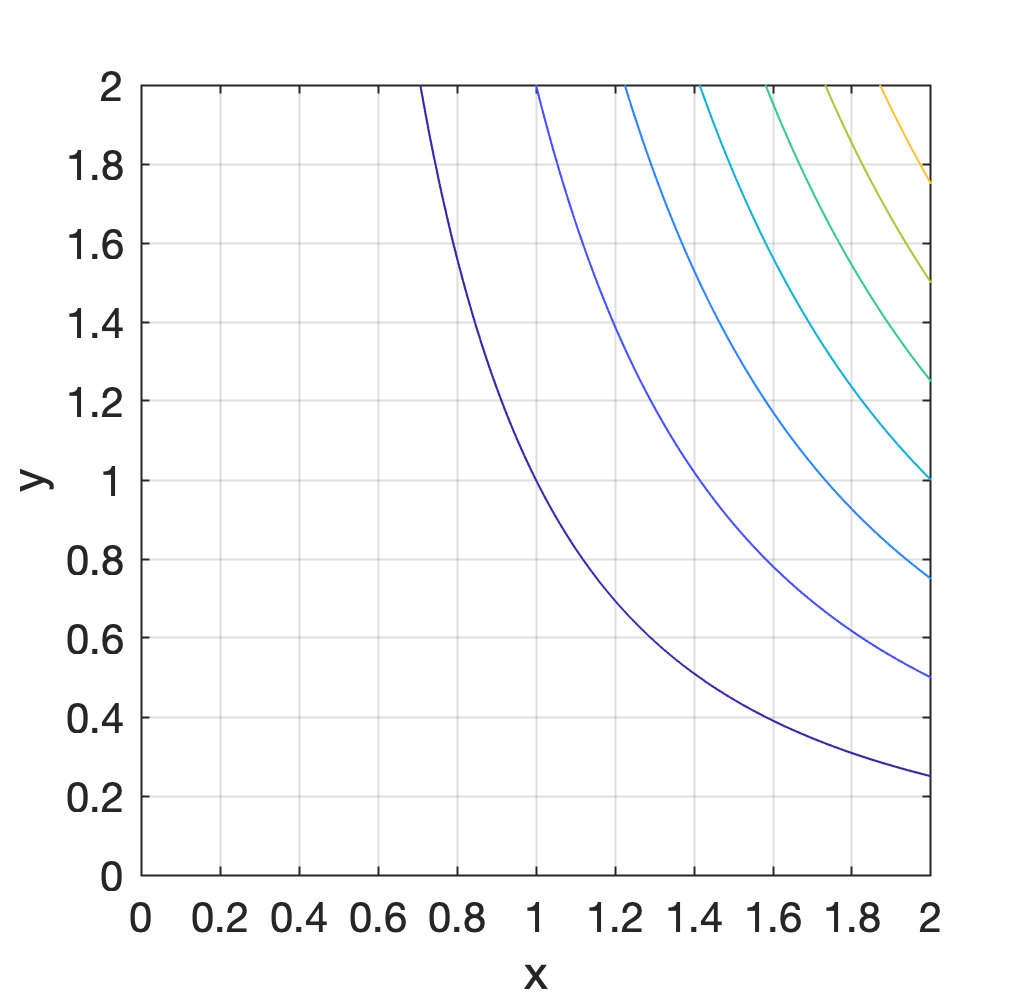
\includegraphics[scale=0.9]{img/C07contour.png}

\item The contour interval is $1$ on the plot above.  Use the contour plot to approximate $\left.Df\right\vert_{(1.4,1)}.$
\end{enumerate}

\vspace{0.2cm}
\hrule
\vspace{0.2cm}

\begin{tcolorbox}
A \textbf{well-posed problem} is one where a solution exists and is unique, and the behavior of the solution changes continuously with change in the initial conditions.  \url{https://en.wikipedia.org/wiki/Well-posed_problem}

In an \textbf{ill-posed problem}, some aspect of well-posedness is violated: the solution might not exist; it might not be unique; it might change discontinuously with change in initial conditions.

For a problem that is not well-posed, it may be possible to reformulate it in a way that is well posed by adding additional assumptions.  The process of reformulation is referred to as \textbf{regularization}.
\end{tcolorbox}

\noindent\textbf{Example.}

``Use the contour plot to approximate $\left.Df\right\vert_{(1.4,1)}.$'' is an ill-posed problem.  There is not a unique solution.

\nocite{*}
\bibliographystyle{unsrt}
\bibliography{biblio}

\end{document}